% Baseline document and packages
\documentclass[aspectratio=169]{beamer}

% Package inclusions
\usepackage[english]{babel}
\usepackage{minted}
\usepackage{multicol}
\usepackage{hyperref}

%% Math packages
\usepackage{amsthm}
\usepackage{amsfonts}
\usepackage{amsmath}
\usepackage{amssymb}
\usepackage{mathtools}
\usepackage{bbm}
\usepackage{physics}
\usepackage{calligra}

\usepackage{csquotes}
\usepackage{tensor}
\usepackage[thicklines]{cancel}
\usepackage{tcolorbox}
\usepackage{pstricks}
\usepackage{etoolbox}
\usepackage[backend=biber, bibstyle=nature, sorting=nty, citestyle=numeric-comp]{biblatex} %Custom bibliography

\DeclareMathAlphabet{\mathcalligra}{T1}{calligra}{m}{n}
\DeclareFontShape{T1}{calligra}{m}{n}{<->s*[2.2]callig15}{}
\newcommand{\scriptr}{\mathcalligra{r}\,}
\newcommand{\boldscriptr}{\pmb{\mathcalligra{r}}\,}
\def\rc{\scriptr}
\def\brc{\boldscriptr}
\def\hrc{\hat\brc}
\newcommand{\ie}{\emph{i.e.}} %id est
\newcommand{\eg}{\emph{e.g.}} %exempli gratia
\newcommand{\rtd}[1]{\ensuremath{\left\lfloor #1 \right\rfloor}}
\newcommand{\dirac}[1]{\ensuremath{\delta \left( #1 \right)}}
\newcommand{\diract}[1]{\ensuremath{\delta^3 \left( #1 \right)}}
\newcommand{\e}{\ensuremath{\epsilon_0}}
\newcommand{\m}{\ensuremath{\mu_0}}
\newcommand{\V}{\ensuremath{\mathcal{V}}}
\newcommand{\prnt}[1]{\ensuremath{\left(#1\right)}} %parentheses
\newcommand{\colch}[1]{\ensuremath{\left[#1\right]}} %square brackets
\newcommand{\chave}[1]{\ensuremath{\left\{#1\right\}}}  %curly brackets
\newcommand\eqdef{\stackrel{\mathclap{\normalfont \tiny\mbox{\textrm{def}}}}{=}}
\useoutertheme{infolines}
\useinnertheme{rectangles}
\usefonttheme{professionalfonts}


% Theme colors
\definecolor{blue2}{HTML}{146FC4}
\definecolor{green2}{HTML}{46C235}
\definecolor{red2}{HTML}{EE4848}
\definecolor{violet2}{HTML}{A647E5}
\definecolor{orange2}{HTML}{FF7425}
\definecolor{darkred}{HTML}{5C2020}
\definecolor{gray}{HTML}{303030}
\definecolor{yellow}{HTML}{f0be52}
\definecolor{brown}{HTML}{975a5a}
\definecolor{lightdarkgold}{HTML}{EEBC1D}

\renewcommand{\CancelColor}{\color{darkred}}

\makeatletter
\newcommand{\mybox}[1]{%
  \setbox0=\hbox{#1}%
  \setlength{\@tempdima}{\dimexpr\wd0+13pt}%
  \begin{tcolorbox}[colback=darkred,colframe=darkred,boxrule=0.5pt,arc=4pt,
      left=6pt,right=6pt,top=6pt,bottom=6pt,boxsep=0pt,width=\@tempdima]
    \textcolor{yellow}{#1}
  \end{tcolorbox}
}
\makeatother

\usecolortheme[named=blue2]{structure}
\usecolortheme{sidebartab}
\usecolortheme{orchid}
\usecolortheme{whale}
\setbeamercolor{titlelike}{parent=structure, bg=structure, fg=white}
\setbeamercolor{section in toc}{fg= white}
\setbeamercolor{subsection in toc}{fg= white}
\setbeamercolor{caption name}{fg=lightdarkgold}

\setbeamercolor{item projected}{bg=yellow, fg = darkred}
\setbeamertemplate{enumerate items}[default]
\setbeamertemplate{navigation symbols}{}
\setbeamercolor{local structure}{fg=yellow}

\setbeamercolor{alerted text}{fg=white}
\setbeamercolor{block title}{bg = blue2}
\setbeamercolor{block title alerted}{bg=red2}
\setbeamercolor{block title example}{bg=green2}
\setbeamercolor{background canvas}{bg=gray}
\setbeamercolor{normal text}{bg=gray,fg=white}


\setbeamertemplate{footline}
        {
      \leavevmode%
      \hbox{%
      \begin{beamercolorbox}[wd=.333333\paperwidth,ht=2.25ex,dp=1ex,center]{author in head/foot}%
        \usebeamerfont{author in head/foot}\insertshortauthor
      \end{beamercolorbox}%
      \begin{beamercolorbox}[wd=.333333\paperwidth,ht=2.25ex,dp=1ex,center]{title in head/foot}%
        \usebeamerfont{title in head/foot}\insertshorttitle
      \end{beamercolorbox}%
      \begin{beamercolorbox}[wd=.333333\paperwidth,ht=2.25ex,dp=1ex,center]{date in head/foot}%
        \usebeamerfont{date in head/foot}\insertshortdate{}%\hspace*{2em}

    %#turning the next line into a comment, erases the frame numbers
        %\insertframenumber{} / \inserttotalframenumber\hspace*{2ex} 

      \end{beamercolorbox}}%
      \vskip0pt%
    }

\setbeamertemplate{headline}
{
    \hbox{
    \begin{beamercolorbox}[wd=.5\paperwidth, ht=2.25ex, dp=1ex, center]{author in head/foot}
    \usebeamerfont{author in head/foot}\insertsection
    \end{beamercolorbox}
    \begin{beamercolorbox}[wd=.5\paperwidth, ht=2.25ex, dp=1ex, center]{title in head/foot}
    \usebeamerfont{title in head/foot}\insertframenumber
    \end{beamercolorbox}
    }
}

\setbeamertemplate{blocks}[rectangle]
\setbeamercovered{dynamic}

\setbeamertemplate{section page}
{
	\begin{centering}
		\begin{beamercolorbox}[sep=27pt,center]{part title}
			\usebeamerfont{section title}\insertsection\par
			\usebeamerfont{subsection title}\insertsubsection\par
		\end{beamercolorbox}
	\end{centering}
}

\setbeamertemplate{subsection page}
{
	\begin{centering}
		\begin{beamercolorbox}[sep=12pt,center]{part title}
			\usebeamerfont{subsection title}\insertsubsection\par
		\end{beamercolorbox}
	\end{centering}
}

% Highlighting colors
\newcommand{\hlight}[1]{\colorbox{violet!50}{#1}}
\newcommand{\hlighta}[1]{\colorbox{darkred!50}{#1}}

\title{The Chrome V8 JavaScript Engine -- A VR perspective}
\subtitle{Internals and Exploitation Patterns of the leading JavaScript Interpreter}
\author[Sam Lovejoy]{\textcolor{yellow}{Sam Lovejoy}}
\institute[IR]{
    \textcolor{white}{Independent Research}%
}
\date{\today}
%%%%%% NOTES CONFIGURATION %%%%%%
% Show notes on right screen
\newtoggle{NOTES}
\newtoggle{DEMO}

\toggletrue{NOTES}
\toggletrue{DEMO}
\iftoggle{NOTES}{\setbeameroption{show notes on second screen=right}}

\begin{document}
    % Introduction included here, all other contents are in their respective files
    \section{Introduction}
    \frame{\titlepage 
        \begin{center}
            Open Source Slides on \href{https://github.com/slovejoy/tech-talks}{\color{pink}https://github.com/slovejoy/tech-talks} \\
            Freely Distributable under CC BY-NC-SA 4.0 License
        \end{center}}
    \begin{frame}{How to Hack V8}
        \tableofcontents
    \end{frame}
    \section{Motivation}
\frame{\sectionpage}

\begin{frame}{Threat Models using Hardware Vulnerabilities}
    Academic researchers have demonstrated CPU vulnerabilities for decades, but the Spectre+Meltdown publications in Jan 2018 introduced them into modern threat models. They can be used in software exploit chains in the following spots,
    \begin{block}{Places in Existing Exploit Chains for CPU Vulnerabilities}
        \begin{itemize}
            \item Local Privilege Escalation (\$250k+)
            \item Browser Sandbox Escapes (\$250k)
            \item Virtualization Escape (\$200k)
            \item Bypasses for security protections like \href{https://arxiv.org/abs/2406.08719}{\color{pink}ARM MTE+PAC}, ASLR, and Intel CET
            \begin{itemize}
                \item Most microarchitectural vulnerabilities tend to yield arbitrary reads across the system.
            \end{itemize}
            \item Pivoting into coprocessors, namely TEEs, but also basebands and DSPs.
       \end{itemize}
    \end{block}
    Even once discovered, it takes around 1 year to patch hardware flaws if they are patched at all. 
    \note{
        \begin{itemize}
            \item Finding hardware bugs is really hard, a few have been found with fuzzing, some by accident, but the majority academics kinda just "conjecture" as try stuff. Sometimes bugs can be gleaned from documentation.
            \item Threat modeling hardware bugs is kinda messed up; in fact, most SoC vendors don't care about instruction-level granularity of code (i.e. they don't care if other folks on the same system know what code you're executing)!
            \item SoC vendors do care that secrets (i.e. dcache) stay protected, such as tokens, keys, and cookies.
            \item See also, the relatively unexplored fingerprinting process.
        \end{itemize}
    }
\end{frame}

\begin{frame}{APT Orchestration of Hardware Vulnerabilities}
    \begin{block}{CVE-2023-38606}
        \begin{itemize}
            \item Exposed GPU MMIO debug registers can disable page protections in the iOS kernel.
            \item The only known hardware vulnerability known ever exploited according to CISA.
            \item Used in \href{https://securelist.com/operation-triangulation-the-last-hardware-mystery/111669/}{\color{pink}{Operation Triangulation Sensation}} against Kaspersky Labs (believed to be USG).
        \end{itemize}
    \end{block}
    Other use cases:
    \begin{itemize}
        \item Stephen Röttger of Google demonstrates that microarchitectural vulnerabilities are useful for escaping the \href{https://googleprojectzero.blogspot.com/2020/02/escaping-chrome-sandbox-with-ridl.html}{\color{pink}{Chrome Sandbox}}.
        \item Carlo Meijer of Midnight Blue uses a \href{https://www.usenix.org/system/files/usenixsecurity23-meijer.pdf}{\color{pink}cache-timing side-channel} to break into the TEE of a Texas Instruments OMAP-L138 SoC. 
    \end{itemize}
    As advanced memory security features become more common, the security landscape will greater reward logical bugs including hardware and microarchitectural flaws. 
    \note{
        \begin{itemize}
            \item It's incredibly hard to detect the exploitation of hardware flaws, there may be some but we just don't know.
            \item In some examples, hardware flaws may be helpful for reverse engineering and introspection as well, not unlike fault injection.
            \item There are tons of papers getting published right now in this field, but not all of these vulnerabilities are practical for exploitation.
        \end{itemize}
    }
\end{frame}
    \section{V8 JavaScript Engine Pipeline}
\frame{\sectionpage}

\begin{frame}{How does V8 work?}
    \begin{block}{V8 is a JIT Compiler for JavaScript and WebAssembly}
    JIT compilers are compilers that profile code as it runs, generating optimizations along the way for "hot" code, or code that runs many times. 
    \end{block}
    \begin{block}{Simplified V8 Pipeline}
        \begin{enumerate}
            \item Parser -- Generate an AST from the JavaScript code
            \item Interpreter -- Named "Ignition", generates an IL representation called Ignition bytecode
            \item Early Compiler -- Named "Maglev", lowers Ignition bytecode into machine code
            \item Optimizing Compiler -- Named "TurboFan", optimizes "hot" machine code with feedback
        \end{enumerate}
    \end{block}
    \note{
        \begin{itemize}
            \item JavaScript is interpreted, not compiled. Lines of code are fed in one at a time.
            \item V8 is an implementation of JavaScript, which itself has specifications associated in ECMAScript. 
            \item Many other parts exist, some are named some are not.
            \item The JIT compiler is historically the most complex and bug-ridden component. It can even be disabled in Chrome now!
        \end{itemize}
    }
\end{frame} 

\begin{frame}
    \begin{figure}
        \centering
        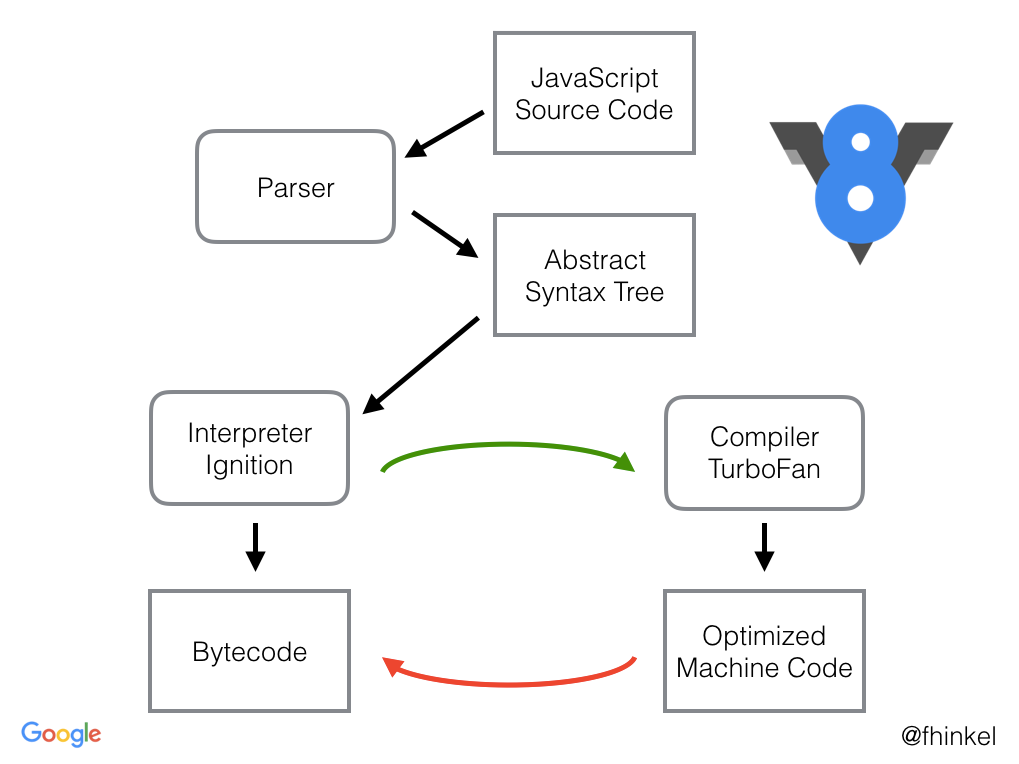
\includegraphics[width=0.6\textwidth]{images/v8-diagram.png}
        \caption{V8 Pipeline Diagram, from Franziska Hinkelmann's \href{https://medium.com/dailyjs/understanding-v8s-bytecode-317d46c94775}{\color{pink}"Understanding V8's Bytecode"}}
    \end{figure}
    \note{
        \begin{itemize}
            \item This diagram is simplified, and from 2017. Notably it does not contain Maglev.
            \item In late 2023 the V8 developers merged the early compiler, Maglev, into mainline.
            \item Regardless of the nyumber of compilers, these process generally stays the same.
            \item All modern javascript engines use multiple stages of compilation now. All are JIT'ed as well.
        \end{itemize}
    }
\end{frame}

\begin{frame}{Ignition}{--print-bytecode}
    Ignition uses the AST from the parser as well as feedback from Turbofan to generate an optimized IL representation.
    \begin{columns}
        \begin{column}{0.5\textwidth}
            \usemintedstyle{vim}
            \inputminted{js}{code/print-bytecode.tex}
        \end{column}
        \begin{column}{0.5\textwidth}
            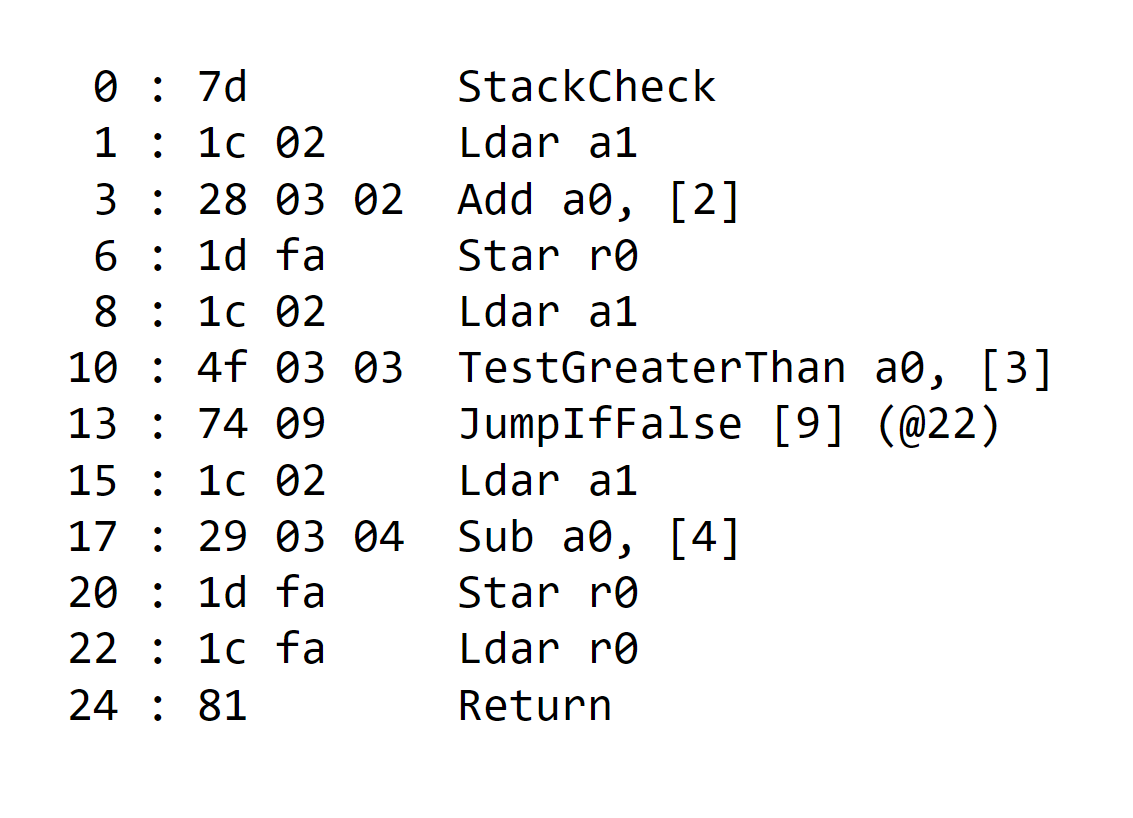
\includegraphics[width=\textwidth]{images/v8-ignition-bytecode.png}
        \end{column}
    \end{columns}
    \note{
        \begin{itemize}
            \item Note the flags to be run on d8, the v8 command line utility.
            \item "Ldar" - Load Accumulator from register (a1, contains arg)
            \item "Add"  - Add register ([2] is argument)
            \item "Star" - Store accumulator into register "result" into r0 
        \end{itemize}
    }
\end{frame}

\begin{frame}{Feedback into Ignition}{--allow-natives-syntax --print-opt-bytecode}
    \begin{columns}
        \begin{column}{0.5\textwidth}
            \usemintedstyle{vim}
            \inputminted{js}{code/ignition-feedback.tex}
        \end{column}
        \begin{column}{0.5\textwidth}
            \begin{itemize}
                \item  As a function runs, Turbofan will provide feedback to Ignition to generate more optimized bytecode. This includes type information, size information, and more! 
                \item Incorrect assumptions lead to a "bailout" which leads to a de-optimization.
                \item This are lots of potential security problems here! The majority of vulnerabilities in V8 occur in the JIT engine!
            \end{itemize}
        \end{column}
    \end{columns}
    \note{
        \begin{itemize}
            \item The first loop contains the body of the function.  
            \item The second for loop contains code that makes the function "hot" (able to be optimized).
            \item The \% sign is to force optimization, which must occur on "hot" functions. \% functions require -allow-natives-syntax. 
            \item Finally, call the function forces the optimization process.
            \item The code here is "dead" for integers, but is important for strings!
        \end{itemize}
    }
\end{frame}

\begin{frame}{Turbofan}{--allow-natives-syntax --trace-turbo}
    \begin{columns}
        \begin{column}{0.33\textwidth}
            \begin{itemize}
                \item Turbofan is the optimizing compiler of V8.
                \item It uses its "Sea of Nodes" to generate a graph from the Ignition bytecode. 
                \item It also translates these nodes into machine code.
                \item Graphs can be visualized using \href{https://chromium.googlesource.com/v8/v8/+/refs/heads/main/tools/turbolizer/}{\color{pink}turbolizer}. 
            \end{itemize}
        \end{column}
        \begin{column}{0.67\textwidth}
            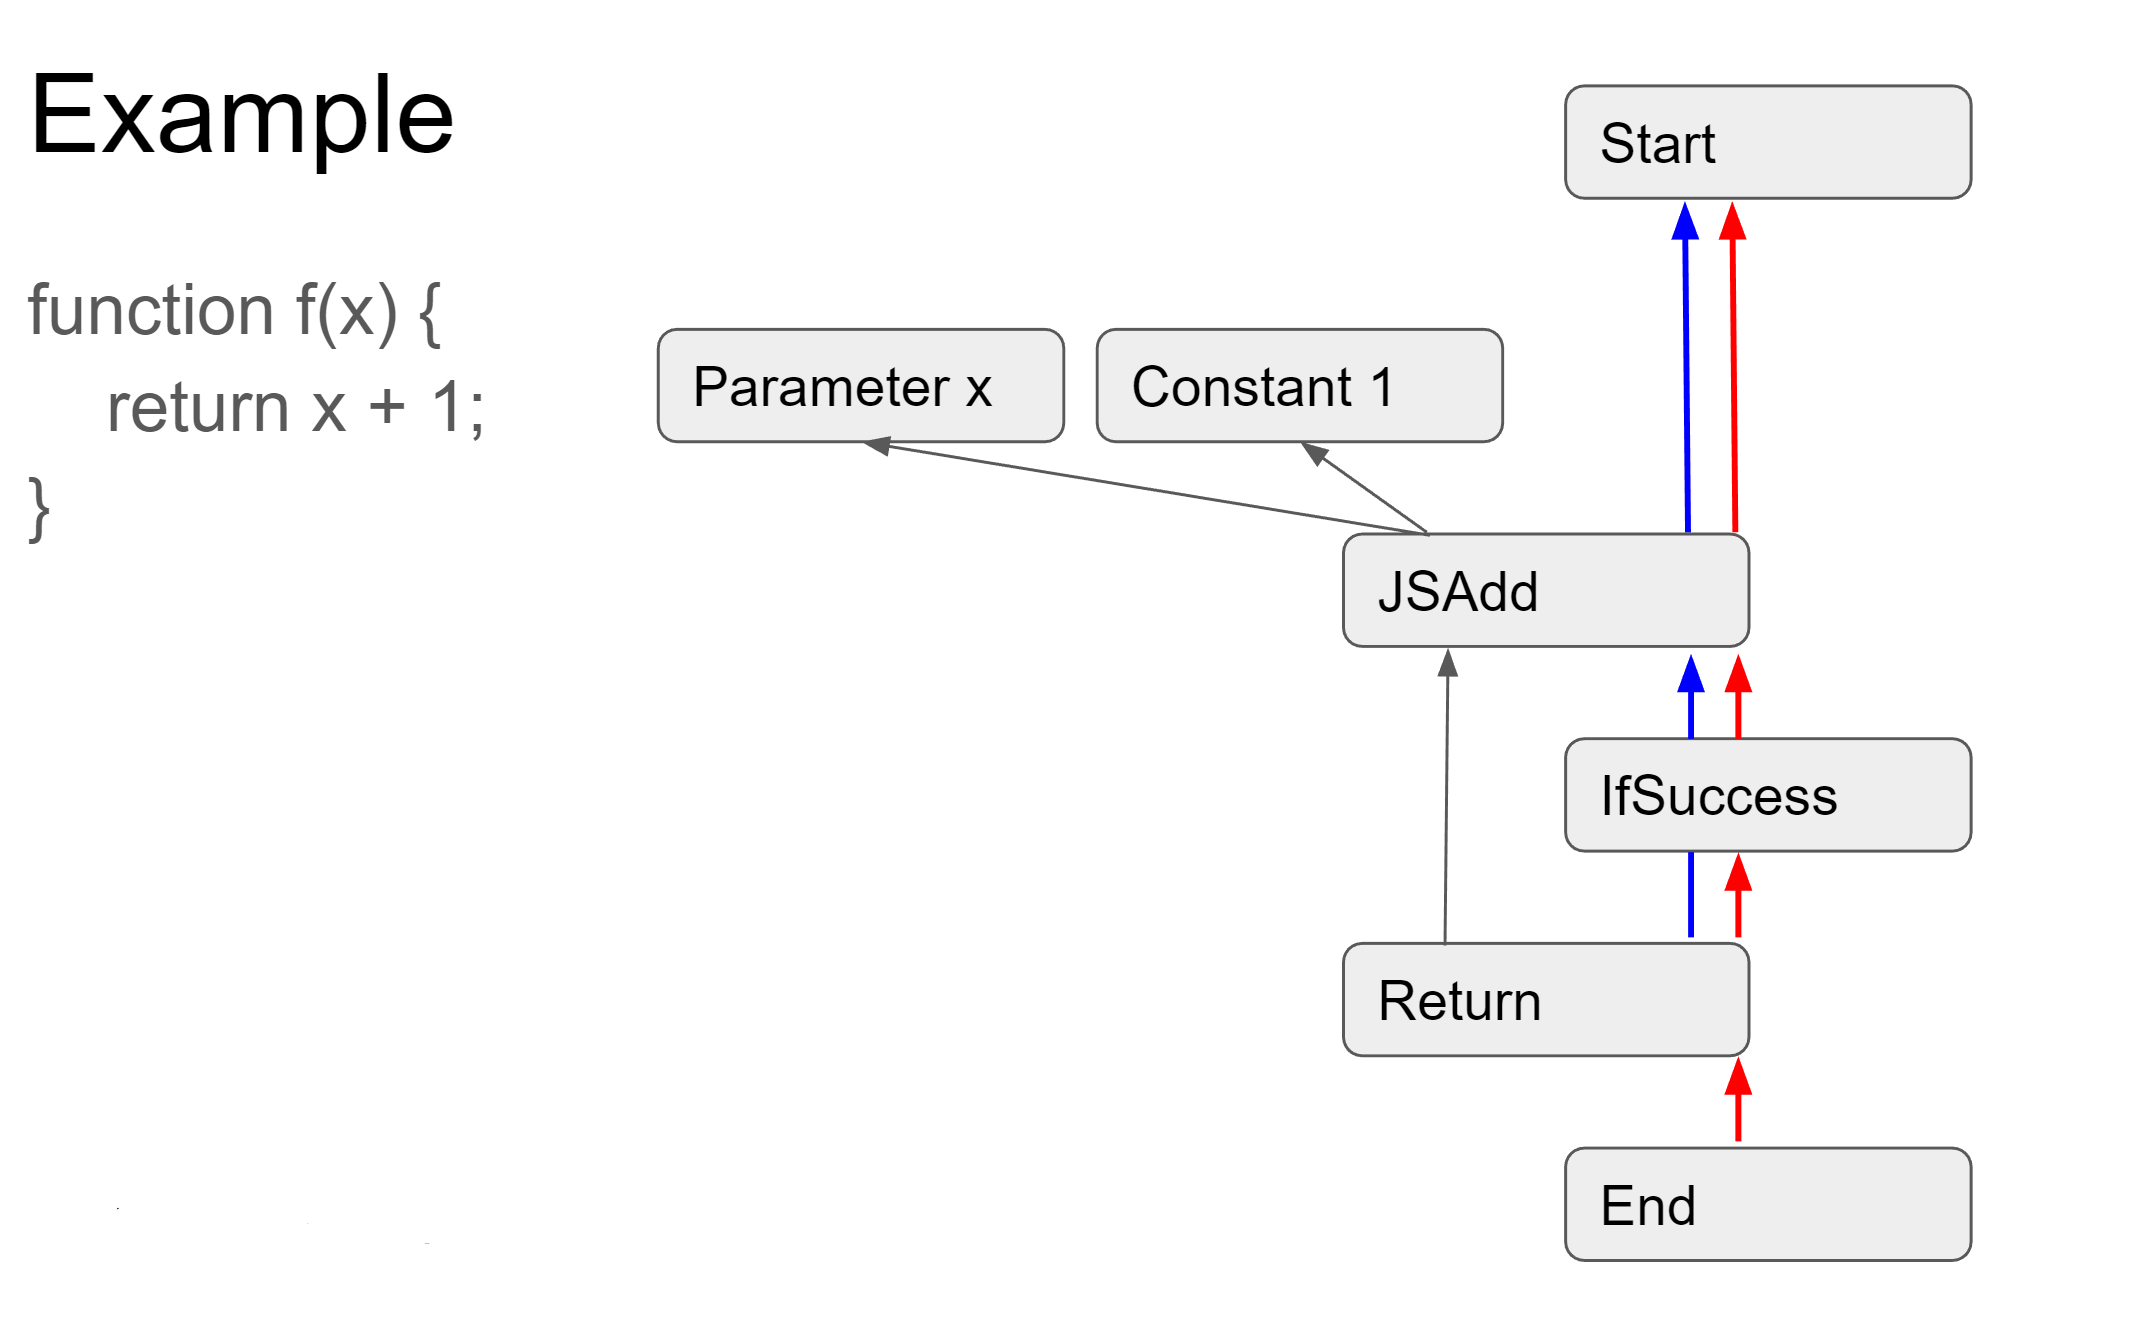
\includegraphics[width=\textwidth]{images/v8-basic-turbo-graph.png}
        \end{column}
    \end{columns}
    \note{
        \begin{itemize}
            \item Turbofan, historically, is the single largest source of exploitable bugs in the V8 engine.
            \item Note that while Turbofan is written in C++, most exploitable bugs in Turbofan and V8 are logical bugs.
            \item This means that a memory-safe implementation of Turbofan/V8 wouldn't really reduce exploitability much. 
        \end{itemize}
    }
\end{frame}

\begin{frame}{The V8 Pointer Cage}
    \begin{columns}
        \begin{column}{0.35\textwidth}
            \begin{itemize}
                \item Introduced in \href{https://v8.dev/blog/v8-release-92}{\color{pink}V8 v9.2}, the pointer cage is a namesake exploit protection employed by the V8 engine.
                \item Pointers in V8 are "sandboxed" to never point outside of the JS Heap. 
                \item Modern pointers are all 32-bit and \textit{tagged} using \href{https://v8.dev/blog/pointer-compression}{\color{pink}pointer compression}.
            \end{itemize}
        \end{column}
        \begin{column}{0.65\textwidth}
            \begin{figure}
                \centering
                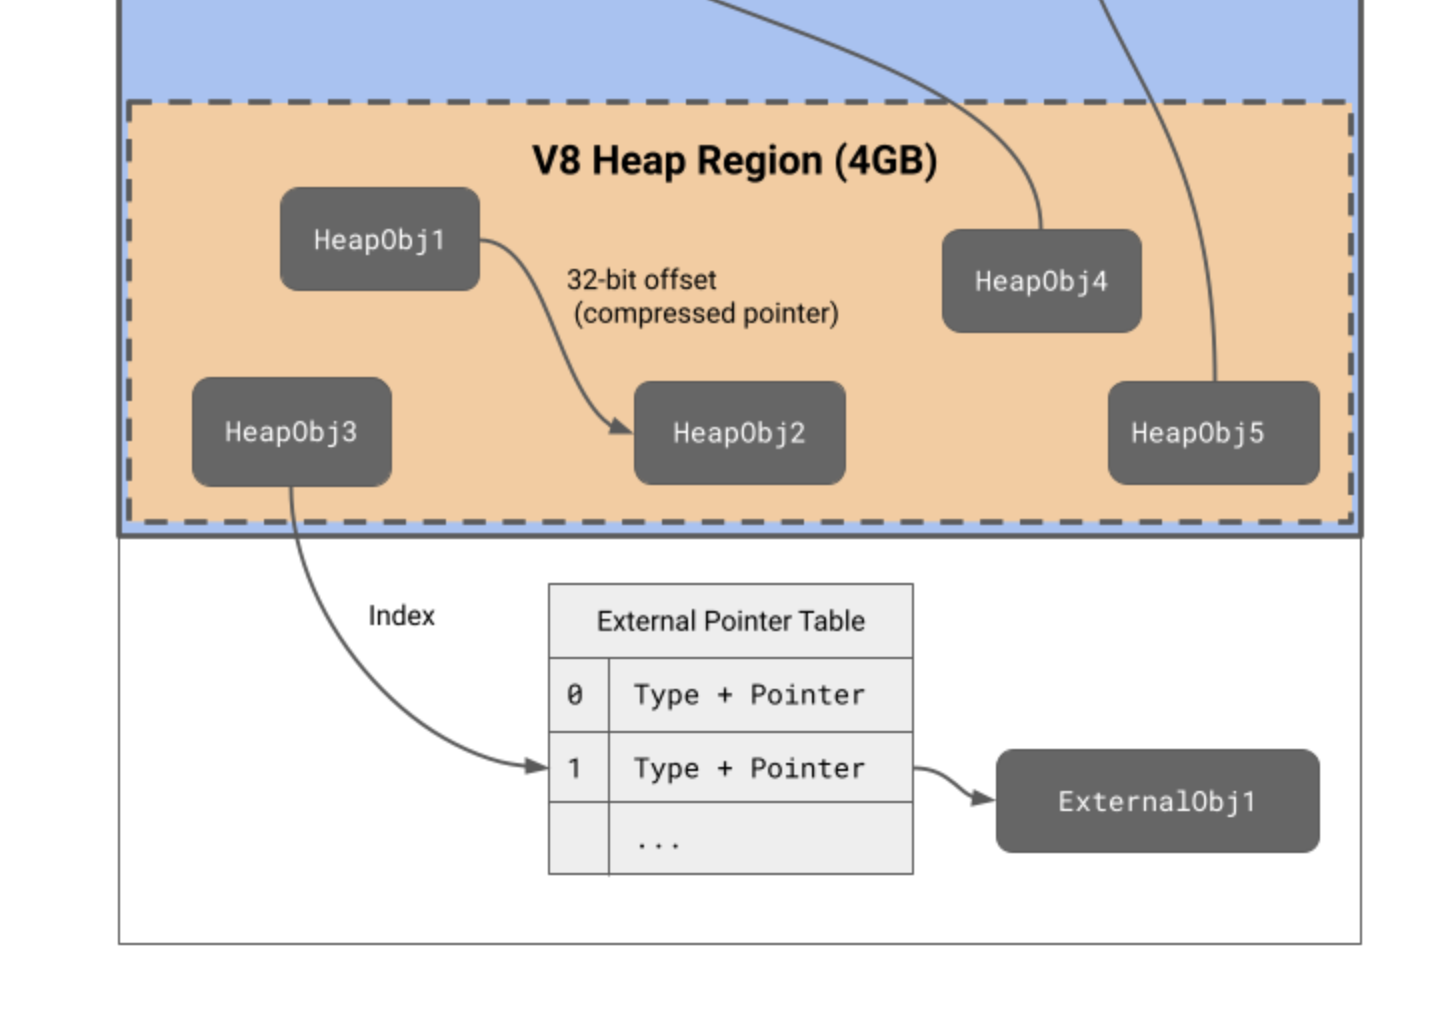
\includegraphics[width=0.80\textwidth]{images/v8-ptr-cage.png}
                \caption{The V8 memory layout with the pointer cage, from RAON.}
                \label{fig:v8-memory-layout}
            \end{figure}
        \end{column}
    \end{columns}
    \note{
        \begin{itemize}
            \item The V8 Pointer cage is the most prominent non-traditional exploit mitigation technique employed by the engine.
            \item Functionally, it eliminates pointers to valid memory addresses from anywhere inside of the heap where JavaScript objects are stored.
            \item Thus, if an attacker can leak memory back into JavaScript variables, they cannot leak pointers to valid memory addresses. 
            \item Tagged pointers are a concept in which the engine stores information about the pointer in its least significant bits.
            \item To do this, V8 assumes that all memory inside its engine is at least 4-byte aligned, giving it 2 bits of metadata it can use on any pointer. The glibc heap also does this.
            \item Other JS implementations use a technique called NaN-boxing, which abuses the IEEE 754 floating point structure.
        \end{itemize}
    }
\end{frame}
    \section{Vulnerability Classes and Notable CVEs}
\frame{\sectionpage}

\begin{frame}{Type Confusion}
    \begin{itemize}
        \item Type Confusion, CWE-843, is a class of vulnerability almost entirely unique to dynamically typed languages such as JavaScript.
        \item A highly exploitable vulnerability class, type confusions almost always lead to remote code execution within the browser sandbox.
        \item They occur as a result of accessing one JS object as if it were another. In V8, object access is determined by its \href{https://v8.dev/docs/hidden-classes}{\color{pink}HiddenClass}.
    \end{itemize}
    \begin{center}
        \begin{figure}
            \centering
            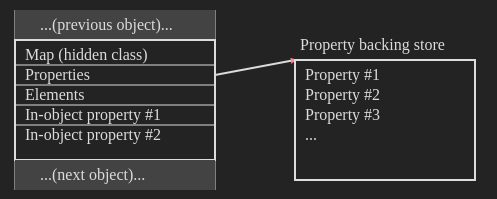
\includegraphics[width=0.5\textwidth]{images/v8-js-object.png}   
            \caption{The memory layout of a JS object, such as with `let v0 = \{\}`.}
            \label{fig:v8-js-object}
        \end{figure}
    \end{center}
    \note{
        \begin{itemize}
            \item Type Confusion is a child of CWE-704, "Improper Type Conversion or Cast"
            \item It is almost like halfway between a logical bug and a memory corruption bug. 
            \item Many bugs, despite not being type confusions, are said to be type confusions in Chrome's security bulletin. 
            \item There are many reasons why a type confusion may occur, but typically they occur due to incorrect graphs in Turbofan.
            \item A HiddenClass is also called a Map, but this has nothing to do with the JavaScript Map() class. 
        \end{itemize}
    }
\end{frame}

\begin{frame}{TheHole}
    \begin{itemize}
        \item TheHole is an internal memory sentinel used by the V8 Engine to represent out-of-bounds, uninitialized, or undefined values.
        \item Before Chrome 114, leaking TheHole into the JavaScript runtime was an extreme security risk. Nowadays, it would require a second vulnerability to fully exploit. 
        \begin{figure}
            \centering
            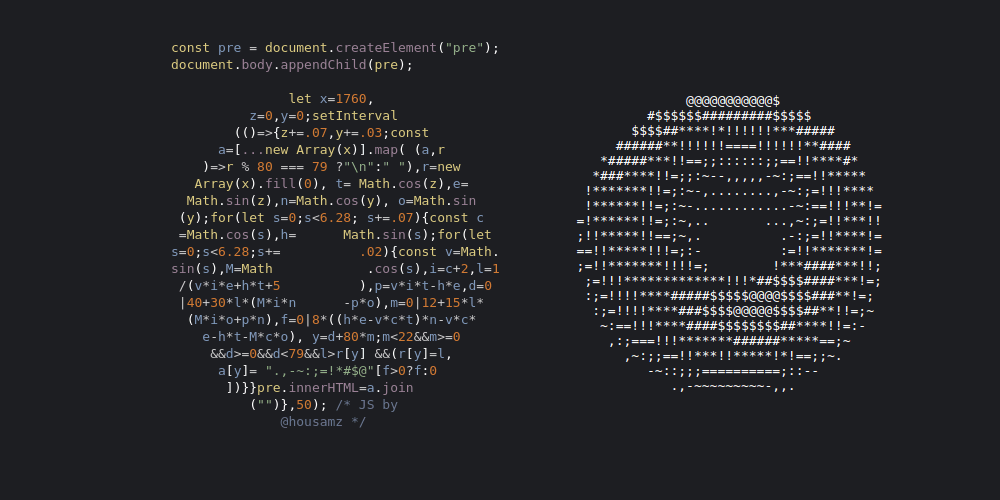
\includegraphics[width=0.55\textwidth]{images/v8-donut.png}
            \caption{A donut made with JavaScript, from Housam Ziad at hmz.ie.}
            \label{fig:donut}
        \end{figure}
    \end{itemize}
    \note{
        \begin{itemize}
            \item TheHole is exploitable for most of Chrome's existance, although the exploit pattern changes over time.
            \item The Chrome Developers didn't realize leaking TheHole was a security issue until Chrome 95 (2021).
            \item TheHole introduced an entire era of Chrome exploitation, lasting about two years (late 2021-2023).
        \end{itemize}
    }
\end{frame}


\begin{frame}{Insufficient Checks in Turbofan in "Array.at" -- BUG 1377775}{V8 Security Team -- Filed by Samuel "saelo" Gro$\beta$}
    \begin{columns}
        \begin{column}{0.5\textwidth}
            \begin{itemize}
                \item This bug runs the built-in function Array.at many times.
                \item Turbofan optimizes the code to expect these objects by inlining the function call to this built-in. 
                \item However, Turbofan only checks the kind of Elements, not the HiddenClass of the objects themselves. 
                \item This leads to a type confusion with "array" and "not\_array". 
            \end{itemize}
        \end{column}
        \begin{column}{0.5\textwidth}
            \usemintedstyle{vim}
            \inputminted{js}{code/buggy-bug.tex}
        \end{column}
    \end{columns}
    \href{https://bugs.chromium.org/p/chromium/issues/detail?id=1377775}{\color{pink}{crbug-1377775}}
    \note{
        \begin{itemize}
            \item This bug is an example of a type confusion. 
            \item The variable "not\_array", is identified by the engine as a JSObject. While "array" has the type JSArray.
            \item Both variables have the same kind of elements, "HOLEY\_ELEMENTS", meaning some members of their array-like backing are undefined. (For example array[1]).
            \item Array.at performs a lookup in the array at index "i". Turbofan sees this and determine that it doesn't need to make the function call to Array.at for the "bug" function. It can just do the lookup provided the types are correct.
            \item In reality, what TurboFan should do is bailout and deoptimize the "bug" function if it is called with exactly the wrong object type. 
            \item This bug was found quite quickly with automated testing and by fuzzing.
        \end{itemize}
    }
\end{frame}

\begin{frame}{Json.stringify Leaks TheHole Value, leading to RCE -- CVE-2021-38003}{Exploited in the wild by Variston -- Filed by Samuel "saelo" Gro$\beta$ and Clement Lecigne of Google TAG}
    \begin{columns}
        \begin{column}{0.5\textwidth}
            \begin{itemize}
                \item Likely the most canonical vulnerability in the history of Chrome, this bug was the first example of an exploit using TheHole. 
                \item The exploit was developed by Variston, a commercial spyware vendor in Barcelona. 
                \item JSON.stringify attempts to serialize a large value, but will ultimately generate an exception. V8 improperly handles the exception, causing an uninitialized value (AKA TheHole) to be returned.
            \end{itemize}
        \end{column}
        \begin{column}{0.5\textwidth}
            \usemintedstyle{vim}
            \inputminted{js}{code/json-stringify.tex}
        \end{column}
    \end{columns}
    \href{https://issues.chromium.org/issues/40057710}{\color{pink}crbug-40057710}
    \note{
        \begin{itemize}
            \item TheHole becomes leaked back into javascript objects most often by out-of-bounds reads. (e.g. bounds-check elimination).
            \item TheHole is a bit like a stack canary or a heap trailer, which are also memory sentinels. 
            \item Prior to Chrome 114, TheHole had an "OddballType" in the V8 engine. It shared this value with booleans and a few other built-in types.
            \item Notably, this allowed functions like toNumber() to be called on TheHole, which is very not good.
            \item Additionally, because of its use as a memory sentinel, other parts of engines were extremely not good at working with it.
            \item Nowadays, TheHole as a dedicated type. And trying to use it in any way causes V8 to halt and catch fire. 
        \end{itemize}
    }
\end{frame}


    \section{Exploitation Patterns}
\frame{\sectionpage}

\begin{frame}{Exploitation of Vulnerabilities in V8 // Chromium}
    \begin{enumerate}
        \item Use the vulnerability to trick V8 into creating an array with an incorrect length. 
        \item Use the corrupted objects to generative out-of-bounds access primitives on the JS Heap. 
        \item With OOB access, create the \textit{addrof} and \textit{fakeobj} primitives for manipulating JS objects. 
        \item Use the \textit{addrof} and \textit{fakeobj} to create arbitrary read and arbitrary write functions.
        \item Gain code execution with the read/write functions via one of
            \begin{itemize}
                \item Overwriting RWX memory from WebAssembly code.
                \item Embed shellcode in JIT-compiled floating point instructions.
                \item Stack pivot from the pointer cage into a version specific ROP chain. 
            \end{itemize}
        \item Pop calculators!
    \end{enumerate}
    \break
    An example PoC showing these can be found below, a full analysis can be found \href{https://faraz.faith/2021-01-07-cve-2020-16040-analysis/}{\color{pink}here}.
    \break
    \href{https://www.exploit-db.com/exploits/49745}{\color{pink}{https://www.exploit-db.com/exploits/49745}}
    \note{
        \begin{itemize}
            \item All vulnerabilities discussed here can be exploited in scripts to 99\%+ certainty.
            \item Unlike in binary exploitation problems, there are no size restrictions, byte restrictions, cache coherenecy, etc.
            \item Exploitation is entirely stateless, and can be restarted easily.
            \item The biggest problem in V8 exploitation is garbage collection, the "invisible" hand that moves memory addresses around.
            \item Exploit patterns evolve rapidly overtime, techniques from even a few months ago are invalid now.
        \end{itemize}
    }
\end{frame}

\begin{frame}{Part 1 -- Create an Array with Incorrect Length}
    \begin{columns}
        \begin{column}{0.5\textwidth}
            \usemintedstyle{vim}
            \inputminted{js}{code/exploit-1.tex}
        \end{column}
        \begin{column}{0.5\textwidth}
            \usemintedstyle{vim}
            \inputminted{js}{code/exploit-1-1.tex}
            \begin{itemize}
                \item This is the implementation of CVE-2020-16040.
                \item It creates an array "arr" with length = -1. 
                \item However, V8 has not adjusted the backing store for that array, leading to OOB access on the JS Heap.
            \end{itemize}
        \end{column}
    \end{columns}
    \note{
        \begin{itemize}
            \item You can't write to the length property directly because it will cause V8 to allocate more memory.
            \item If you trick the engine with an OOB write, V8 will assume the array is longer but won't allocate more memory. 
            \item This vulnerability is not really a type confusion, but the underlying issue does lie within Turbofan.
            \item Turbofan mathematically (and incorrectly) proves that the function 'vuln' can never allocate an array with nonzero length.
            \item The for loop triggers Turbofan's JIT compilation of the 'vuln' function, and insufficent deoptimizations occur in the vuln(false) function call. 
        \end{itemize}
    }
\end{frame}

\begin{frame}{Part 2 -- Creating OOB access on the JS Heap}
    \begin{columns}
        \begin{column}{0.5\textwidth}
            \usemintedstyle{vim}
            \inputminted[]{js}{code/exploit-2.tex}
            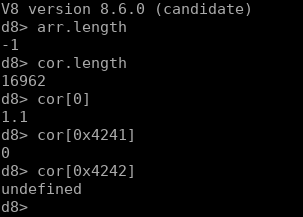
\includegraphics[width=\textwidth]{images/v8-length-screenshot.png}
        \end{column}
        \begin{column}{0.5\textwidth}
            \begin{itemize}
                \item In this snippet, "offset" represents the distance in memory from "arr" to "cor" on the JS heap. 
                \item This snippet uses out-of-bounds access via "arr" to modify the metadata of "cor".
                \item This overwrites the length of "cor" to be 0x4242, which grants OOB access on the JS Heap. 
            \end{itemize}
        \end{column}
    \end{columns}
    \note{
        \begin{itemize}
            \item This part of the exploit isn't really necessary, since the array length of 'arr' is already corrupted. 
            \item However, it nicely illustrates the OOB access. 
            \item Note that if garbage collection happens unexpectedly, the OOB access can get messed up! 
        \end{itemize}
    }
\end{frame}

\begin{frame}{Part 3 -- Create the \textit{addrof} and \textit{fakeobj} primitives}
    \begin{columns}
        \begin{column}{0.5\textwidth}
            \usemintedstyle{vim}
            \inputminted[]{js}{code/exploit-3.tex}
        \end{column}
        \begin{column}{0.5\textwidth}
            \begin{itemize}
                \item "addrof" is a function this takes in an arbitrary JS object \textit{k}. Using "arr" OOB write, insert \textit{k} into "cor" (replacing 1.1). Then, read the object from "cor". This will read the pointer to \textit{k} as it were a float. 
                \item "fakeobj" is the opposite of addrof; rather than leak pointers to the JS runtime, it allows the JS runtime to insert arbitrary values that V8 will interpret as a pointer. 
            \end{itemize}
        \end{column}
    \end{columns}
    \note{
        \begin{itemize}
            \item 'addrof' and 'fakeobj' originally come from a phrack article written by Samuel GroB, former project-zero now the head of the V8 security team.
            \item The premise here is that OOB access by one object doesn't update the HiddenClass of another. So if one uses 'arr' to write into 'cor'. The engine still thinks that 'cor' is an Array of floating point numbers. Thus, the memory address of the object will be returned as a floating point value. 
            \item Note, this would NOT work if the pointer cage was in place! Since valid pointers do not exist on the heap (unless they point to other things also on the heap)!
            \item fakeobj tricks the V8 engine into thinking some blob of memory is actually a JavaScript object. It is helpful for gaining arbitrary writes. 
        \end{itemize}
    }
\end{frame}

\begin{frame}{Part 4 -- Create Arbitrary Read and Arbitrary Write Functions}
    \begin{columns}
        \begin{column}{0.5\textwidth}
            \usemintedstyle{vim}
            \inputminted[]{js}{code/exploit-4.tex}
        \end{column}
        \begin{column}{0.5\textwidth}
            \begin{itemize}
                \item The first three lines:
                    \begin{itemize}
                        \item Read the HiddenClass for the built-in Array type using OOB access
                        \item Create a legitimate object "arr2" which contains the array map 
                        \item Create an illegitimate object "fake" using the array contents of "arr2" 
                    \end{itemize}
                \item For both functions, arr2[1] points to the fake's \textit{backing store}, that is, the memory location where the contents of "fake" are stored. 
            \end{itemize}
        \end{column}
    \end{columns}
    \note{
        \begin{itemize}
            \item In this version of V8, the metadata of a JSArray object has a pointer inside of its metadata called the "backing store". 
            \item This "backing store" pointer points to a memory region that contains enough space to contain the elements of the array.
            \item However, if the "backing store" pointer were to become corrupted by an attacker, then an attacker can use that array in JS to obtain arbitrary read and write locations.
            \item To do this, leak the base address of the JSArray object using `addrof`. Then set its backing store to the argument `addr`, then, read/write to the address and return its value. 
            \item In practice, its best to restore the original backing store of the Array, otherwise triggering garbage collection can crash the engine. 
        \end{itemize}
    }
\end{frame}

\begin{frame}{Part 5 -- Allocate a RWX Page using WebAssembly}
    \usemintedstyle{vim}
    \inputminted[]{js}{code/exploit-5.tex}
    \begin{center}
        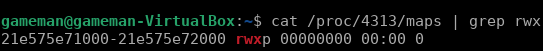
\includegraphics[width=0.8\textwidth]{images/v8-memory-rwx.png}
    \end{center}
    \break
    \begin{itemize}
        \item In this version of Chrome, WebAssembly functions will allocate RWX memory by default.
        \item In late 2021, V8 started toggling WASM code pages between writable and executable. 
        \item Recently, V8 developers introduced an additional sandbox on the JS Heap.
    \end{itemize}
    \note{
        \begin{itemize}
            \item WebAssembly is special type of assembly code generated by compiled languages to run in a browser context.
            \item In this version of Chrome, webassembly code lives in directly accesible RWX memory. 
            \item This RWX memory didn't see any kind of additional protections until 2021!
            \item This illustrates how while bugs in V8 haven't changed much, in reality the exploit patterns have become significantly harder.
        \end{itemize}
    }
\end{frame} 

\begin{frame}{Part 6 -- Overwrite the contents of the RWX pages}
    \begin{columns}
        \begin{column}{0.5\textwidth}
            \usemintedstyle{vim}
            \inputminted[]{js}{code/exploit-6.tex}
        \end{column}
        \begin{column}{0.5\textwidth}
            \begin{itemize}
                \item Leak the address of the WebAssembly instance using \textit{addrof}.
                \item A pointer to the RWX page will be at offset 0x68 from the leaked address. 
                \item Dereference that pointer using \textit{arbread}. 
                \item Copy some shellcode into the body of that rwx page and pop a calc!
            \end{itemize}
        \end{column}
    \end{columns}
    \note{
        \begin{itemize}
            \item Since the V8 exploit destabilizes the renderer process in the browser, exploit engineering beyond a PoC largely involves stabilizing the browser. 
            \item Note that normal shellcode here won't work in a browser because of the seccomp-bpf sandbox.
            \item The renderer is restricted to a small number of system calls it is allowed to make, execve is not one of them.
            \item However, running the exploit in d8, the command line version of V8, will work fine. 
        \end{itemize}
    }
\end{frame}

\begin{frame}{Part 7 -- Pop a calc!}
    \centering
        \Huge\bfseries
    \textcolor{yellow}{Calculator time!}
    \note{
        \begin{itemize}
            \item If running in Chrome on Linux, the "--no-sandbox" flag should be passed on the command line.
            \item To verify the sandbox is off, use "chrome://sandbox" in the URL.
            \item The exploit needs to be packaged as an HTML document to work properly.
            \item Chrome versions and V8 versions are directly correlated. V8 9.2 -> Chrome 92.
            \item Google publishes all commits to V8 and Chromium via CI/CD. One can freely download these and test on.
        \end{itemize}
    }
\end{frame}
    \section{Conclusion}
\begin{frame}{}
    \centering
        \Huge\bfseries
    \textcolor{yellow}{Questions?}
    \note{
        \begin{itemize}
            \item This is mostly a hobby presentation, I just think these vulnerabilities are cool. I haven't really worked on much these ever at all.
        \end{itemize}
    }
\end{frame}

% Flush+Reload
% Foreshadowz
% RIDL
% Spectre
% TikTag
% Zenbleed
    \iftoggle{LAB}{\section{LAB}
\begin{frame}{}
    \centering
        \Huge\bfseries
    \textcolor{yellow}{LAB}
\end{frame}

\begin{frame}{Promise.Any.Call leaks ``TheHole" Value -- CVE-2022-4174}{Discovered by Zhenghang ``kiprey" Xiao -- Independent Security Researcher}
    \begin{columns}
        \begin{column}{0.55\textwidth}
            \begin{itemize}
                \item This bug functionally behaves identical to Json.stringify's hole leak.
                \item There are plenty of exploits for TheHole online. 
                \item Download a specific version from \href{https://commondatastorage.googleapis.com/v8-asan/index.html}{\color{pink}here}.
                    \begin{itemize}
                        \item Version '77090' will work for this exploit.
                        \item Use 'linux-release' to pop a calculator.
                        \item Use 'linux-debug' when not trying to exploit.
                        \item Use '--gdbjit-full' in your command line! 
                    \end{itemize}
            \end{itemize}
        \href{https://bugs.chromium.org/p/chromium/issues/detail?id=1379054}{\color{pink}{crbug-1379054}} \\
        Try it yourself! Try and understand every line of code by leaving a comment. 
        \end{column}
        \begin{column}{0.4\textwidth}
            \usemintedstyle{vim}
            \inputminted{js}{code/promise.tex}
        \end{column}
    \end{columns}
    \note{
        \begin{itemize}
            \item Promise.Any.Call was patched in Chrome 106.
            \item This vulnerability is exploitable from Chrome 86-106.
            \item Zhenghang Xiao is still an active Chrome VRP researcher, ranking 3rd in bug bounties in Chrome.
            \item He has a black hat talk, it's pretty cool. 
        \end{itemize}
    }
\end{frame}
}{}
    \iftoggle{CUT-CONTENT}{\begin{frame}{}
    \centering
        \Huge\bfseries
    \textcolor{yellow}{Deleted Scenes}
\end{frame}

\begin{frame}{Notable Individuals in the V8 0-day Research Community}
    \begin{itemize}
        \item Samuel Gro$\beta$ -- Head of V8 Security Team, former Google Project Zero
        \item Clement Lecigne -- Google Threat Analysis Group, who has ``burned" many 0-days in V8 
        \item Hossein Lotfi -- Zero-day Initiative, amazing documentation about V8 from Pwn2Own 
        \item Man Yue Mo -- GitHub Security Lab, great writeups about 0-day Vulnerabilities 
        \item Zhenghang Xiao -- Independent Security Researcher speaking at Black Hat 2023
        \item Alisa Esage -- Independent Security Researcher with great YouTube talk
    \end{itemize}
    \break
    \href{https://phrack.org/issues/70/3.html}{\color{pink}{Samuel Grob's phrack.org article on V8 exploitation}}
    \break
    \href{https://www.youtube.com/watch?v=WouAptHlyC4}{\color{pink}{Alisa Esage's Modern Attacks on Google Chrome YouTube talk}}
\end{frame}

\begin{frame}{Type Confusion in Value Serializer -- CVE-2023-1214}{Discovered by Man Yue Mo of GitHub Security Lab}
    \begin{columns}
        \begin{column}{0.7\textwidth}
            \begin{itemize}
                \item This vulnerability involves incorrect assumptions made during a Map (HiddenClass) transition.
                \item Many objects in JavaScript are likely to be the same, so V8 saves on memory by re-using object mappings.
                \item Maps will point to other maps, forming a tree.
                \item Map transitions occur when new properties are added or removed from objects creating a ``never-before-seen" layout. 
            \end{itemize}
        \href{https://bugs.chromium.org/p/chromium/issues/detail?id=1412487}{\color{pink}{crbug-1412487}}
        \end{column}
        \begin{column}{0.3\textwidth}
            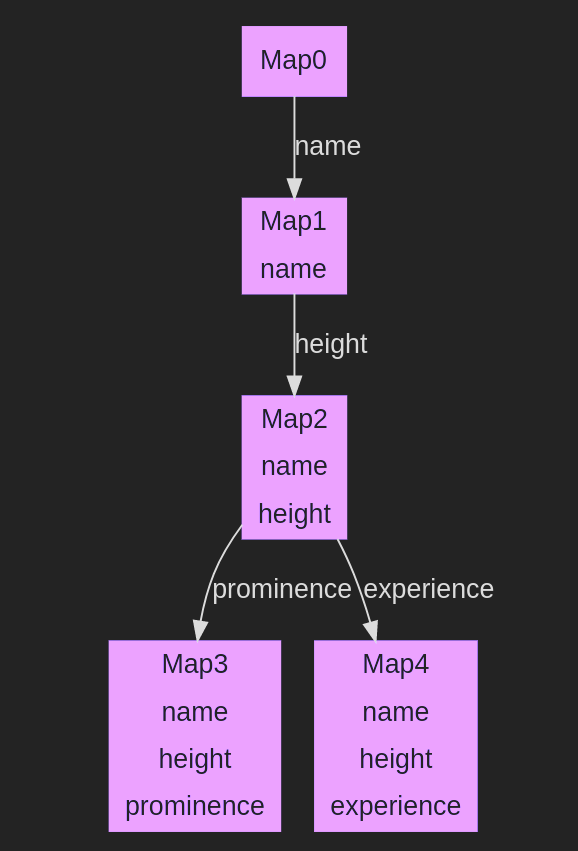
\includegraphics[height=6.5cm]{images/v8-hiddenclass.png}
        \end{column}
    \end{columns}
\end{frame}

\begin{frame}[fragile]{Type Confusion Example}
    \begin{columns}
        \begin{column}{0.5\textwidth}
            \usemintedstyle{vim}
            \inputminted{C}{code/type-confusion.tex}
        \end{column}
        \begin{column}{0.5\textwidth}
            \usemintedstyle{vim}
            \inputminted{C}{code/type-confusion-exploit.tex}
        \end{column}
    \end{columns}
\end{frame}}{}
\end{document}
